\section{Desain Sistem}
\label{sec:desainsistem}

\subsection{Desain Robot yang Digunakan}

\begin{figure} [ht]
  \centering
  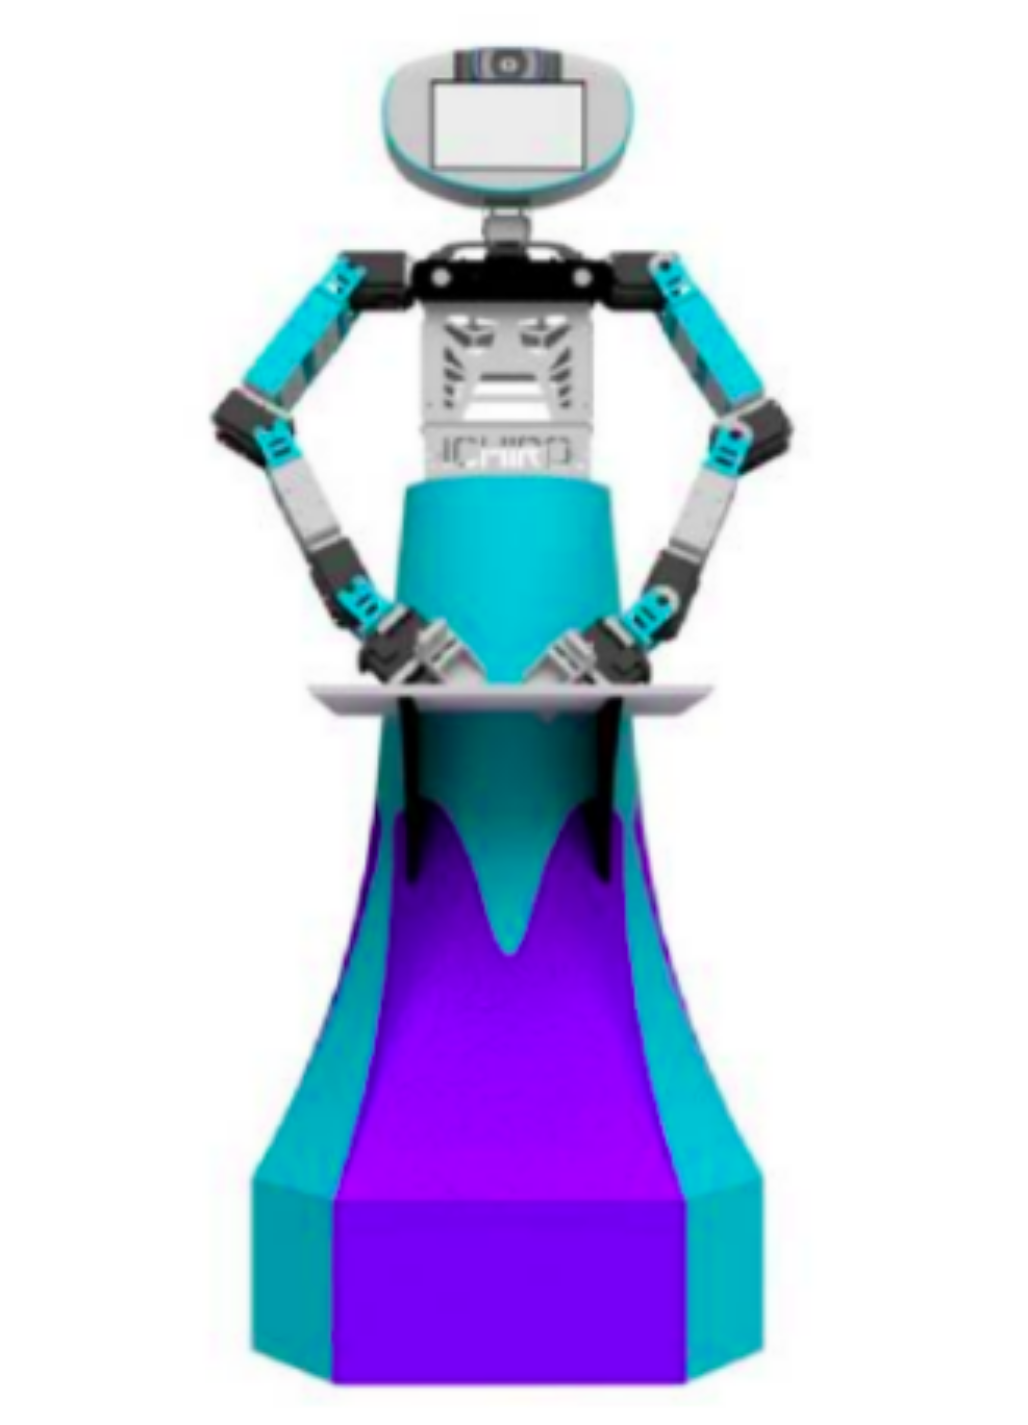
\includegraphics[scale=0.6]{gambar/desainrobot.png}
  \caption{Diagram desain robot \emph{Dienen}.}
  \label{fig:desainrobot}
\end{figure}

Robot yang akan digunakan pada pada penelitian ini adalah robot \emph{Dienen} yang merupakan kelanjutan dari robot \emph{IRIS} \citep{dikairono2020}\citep{zanuar2019} dengan penambahan desain dari robot \emph{ICHIRO} \citep{muhtadin2019} di bagian atas robot.
Desain seperti ini secara umum dikenal sebagai desain \emph{mobile humanoid robot} \citep{mohamed2012}, yang merupakan desain gabungan antara robot mobile dan robot humanoid.
Seperti yang terlihat pada Gambar \ref{fig:desainrobot}, bagian bawah robot menyerupai robot mobile dengan penggerak \emph{omnidirectional wheels} yang memungkinkan pergerakan robot secara \emph{holonomic} ke segala arah\citep{oliveira2008}, sedangkan bagian atas robot menyerupai robot humanoid yang terdiri atas badan, kepala, dan lengan.
Dengan desain mobile humanoid robot ini, diharapkan pengguna bisa merasakan interaksi sosial yang lebih baik dengan robot karena memiliki bentuk mendekati manusia \citep{rossi2018} sekaligus mempermudah navigasi dari robot ke berbagai tempat.

Robot \emph{Dienen} dilengkapi dengan beberapa sensor seperti IMU (\emph{inertial measurement unit}) untuk mengetahui orientasi dari robot, \emph{rotary encoder} untuk melakukan perhitungan odometri dari robot, \emph{distance sensor} untuk mendeteksi adanya objek lain di sekitar robot, sensor kamera di kepala untuk menangkap citra, dan sensor \emph{depth camera} yang nantinya bisa digunakan untuk melakukan mapping dari ruangan.
Selain itu robot ini juga dilengkapi dengan dua lengan seperti robot manipulator yang bisa diatur pada berbagai posisi dan orientasi \citep{iqbal2012}.
Dengan adanya sensor dan aktuator ini diharapkan robot mampu melakukan tindakan \emph{assistive} secara sosial sesuai dengan data yang didapatkan dari sensor yang ada.

\subsection{Desain Kontroler Robot}

\begin{figure} [ht]
  \centering
  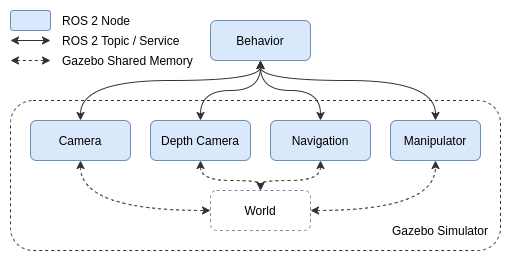
\includegraphics[scale=0.45]{gambar/kontrolersimulasi.png}
  \caption{Diagram sistem kontroler robot di simulasi.}
  \label{fig:kontrolersimulasi}
\end{figure}

Kontroler robot yang digunakan untuk simulasi ini akan dikembangkan menggunakan ROS 2.
Kontroler tersebut akan dipisah menjadi beberapa bagian dalam bentuk \emph{ROS 2 node} seperti yang terlihat pada Gambar \ref{fig:kontrolersimulasi}.
Setiap node yang ada akan terhubung satu sama lain menggunakan sistem komunikasi antar proses ROS 2 yang berupa \emph{topics} dan \emph{services}.

Bagian utama dari kontroler robot tersebut adalah \emph{node behavior} yang berisi program yang mengatur segala tindakan robot berdasarkan data yang didapat dari sensor yang ada di simulasi.
Kemudian node Behavior tersebut akan terhubung dengan empat node lain yang merepresentasikan sensor dan aktuator yang ada pada robot.
Keempat node tersebut akan terpasang di dalam cakupan simulator Gazebo sebagai \emph{Gazebo plugins}, sehingga mampu digunakan untuk mengakses dan memanipulasi data yang ada di simulasi menggunakan sistem \emph{shared memory} pada Gazebo \citep{gazeboplugins}.

\begin{figure} [ht] \centering
  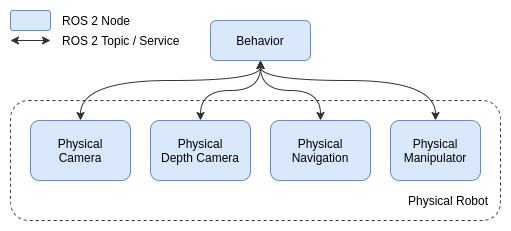
\includegraphics[scale=0.45]{gambar/kontrolerfisik.png}
  \caption{Diagram sistem kontroler robot untuk robot fisik.}
  \label{fig:kontrolerfisik}
\end{figure}

Sistem ini dirancang secara terpisah agar \emph{node Behavior} yang diujikan di lingkungan simulasi bisa langsung bekerja pada robot fisik.
Seperti yang terlihat pada Gambar \ref{fig:kontrolerfisik}, transfer kontroler ke robot fisik dapat dilakukan dengan mengubah keseluruhan cakupan yang ada di simulator Gazebo, yang berupa empat node yang telah disebutkan sebelumnya, menjadi node yang memproses sensor dan aktuator yang ada pada robot fisik.
Dengan ini pengujian yang dilakukan di simulasi bisa langsung diterapkan ketika diujikan pada robot fisik karena tidak perlunya pembuatan ulang kontroler yang menyesuaikan sistem yang ada pada robot.
